%% bare_jrnl.tex
%% V1.4b
%% 2015/08/26
%% by Michael Shell
%% see http://www.michaelshell.org/
%% for current contact information.
%%
%% This is a skeleton file demonstrating the use of IEEEtran.cls
%% (requires IEEEtran.cls version 1.8b or later) with an IEEE
%% journal paper.
%%
%% Support sites:
%% http://www.michaelshell.org/tex/ieeetran/
%% http://www.ctan.org/pkg/ieeetran
%% and
%% http://www.ieee.org/

%%*************************************************************************
%% Legal Notice:
%% This code is offered as-is without any warranty either expressed or
%% implied; without even the implied warranty of MERCHANTABILITY or
%% FITNESS FOR A PARTICULAR PURPOSE! 
%% User assumes all risk.
%% In no event shall the IEEE or any contributor to this code be liable for
%% any damages or losses, including, but not limited to, incidental,
%% consequential, or any other damages, resulting from the use or misuse
%% of any information contained here.
%%
%% All comments are the opinions of their respective authors and are not
%% necessarily endorsed by the IEEE.
%%
%% This work is distributed under the LaTeX Project Public License (LPPL)
%% ( http://www.latex-project.org/ ) version 1.3, and may be freely used,
%% distributed and modified. A copy of the LPPL, version 1.3, is included
%% in the base LaTeX documentation of all distributions of LaTeX released
%% 2003/12/01 or later.
%% Retain all contribution notices and credits.
%% ** Modified files should be clearly indicated as such, including  **
%% ** renaming them and changing author support contact information. **
%%*************************************************************************


% *** Authors should verify (and, if needed, correct) their LaTeX system  ***
% *** with the testflow diagnostic prior to trusting their LaTeX platform ***
% *** with production work. The IEEE's font choices and paper sizes can   ***
% *** trigger bugs that do not appear when using other class files.       ***                          ***
% The testflow support page is at:
% http://www.michaelshell.org/tex/testflow/



\documentclass[journal]{IEEEtran}
%
% If IEEEtran.cls has not been installed into the LaTeX system files,
% manually specify the path to it like:
% \documentclass[journal]{../sty/IEEEtran}





% Some very useful LaTeX packages include:
% (uncomment the ones you want to load)


% *** MISC UTILITY PACKAGES ***
%
%\usepackage{ifpdf}
% Heiko Oberdiek's ifpdf.sty is very useful if you need conditional
% compilation based on whether the output is pdf or dvi.
% usage:
% \ifpdf
%   % pdf code
% \else
%   % dvi code
% \fi
% The latest version of ifpdf.sty can be obtained from:
% http://www.ctan.org/pkg/ifpdf
% Also, note that IEEEtran.cls V1.7 and later provides a builtin
% \ifCLASSINFOpdf conditional that works the same way.
% When switching from latex to pdflatex and vice-versa, the compiler may
% have to be run twice to clear warning/error messages.






% *** CITATION PACKAGES ***
%
%\usepackage{cite}
% cite.sty was written by Donald Arseneau
% V1.6 and later of IEEEtran pre-defines the format of the cite.sty package
% \cite{} output to follow that of the IEEE. Loading the cite package will
% result in citation numbers being automatically sorted and properly
% "compressed/ranged". e.g., [1], [9], [2], [7], [5], [6] without using
% cite.sty will become [1], [2], [5]--[7], [9] using cite.sty. cite.sty's
% \cite will automatically add leading space, if needed. Use cite.sty's
% noadjust option (cite.sty V3.8 and later) if you want to turn this off
% such as if a citation ever needs to be enclosed in parenthesis.
% cite.sty is already installed on most LaTeX systems. Be sure and use
% version 5.0 (2009-03-20) and later if using hyperref.sty.
% The latest version can be obtained at:
% http://www.ctan.org/pkg/cite
% The documentation is contained in the cite.sty file itself.






% *** GRAPHICS RELATED PACKAGES ***
%
\ifCLASSINFOpdf
\usepackage[pdftex]{graphicx}
  % declare the path(s) where your graphic files are
\graphicspath{{./drawings/}}
% \graphicspath{{../pdf/}{../jpeg/}}
  % and their extensions so you won't have to specify these with
  % every instance of \includegraphics
  %\DeclareGraphicsExtensions{.pdf,.jpeg,.png}
\else
  % or other class option (dvipsone, dvipdf, if not using dvips). graphicx
  % will default to the driver specified in the system graphics.cfg if no
  % driver is specified.
  % \usepackage[dvips]{graphicx}
  % declare the path(s) where your graphic files are
  % \graphicspath{{../eps/}}
  % and their extensions so you won't have to specify these with
  % every instance of \includegraphics
  % \DeclareGraphicsExtensions{.eps}
\fi
% graphicx was written by David Carlisle and Sebastian Rahtz. It is
% required if you want graphics, photos, etc. graphicx.sty is already
% installed on most LaTeX systems. The latest version and documentation
% can be obtained at: 
% http://www.ctan.org/pkg/graphicx
% Another good source of documentation is "Using Imported Graphics in
% LaTeX2e" by Keith Reckdahl which can be found at:
% http://www.ctan.org/pkg/epslatex
%
% latex, and pdflatex in dvi mode, support graphics in encapsulated
% postscript (.eps) format. pdflatex in pdf mode supports graphics
% in .pdf, .jpeg, .png and .mps (metapost) formats. Users should ensure
% that all non-photo figures use a vector format (.eps, .pdf, .mps) and
% not a bitmapped formats (.jpeg, .png). The IEEE frowns on bitmapped formats
% which can result in "jaggedy"/blurry rendering of lines and letters as
% well as large increases in file sizes.
%
% You can find documentation about the pdfTeX application at:
% http://www.tug.org/applications/pdftex





% *** MATH PACKAGES ***
%
%\usepackage{amsmath}
% A popular package from the American Mathematical Society that provides
% many useful and powerful commands for dealing with mathematics.
%
% Note that the amsmath package sets \interdisplaylinepenalty to 10000
% thus preventing page breaks from occurring within multiline equations. Use:
%\interdisplaylinepenalty=2500
% after loading amsmath to restore such page breaks as IEEEtran.cls normally
% does. amsmath.sty is already installed on most LaTeX systems. The latest
% version and documentation can be obtained at:
% http://www.ctan.org/pkg/amsmath





% *** SPECIALIZED LIST PACKAGES ***
%
%\usepackage{algorithmic}
% algorithmic.sty was written by Peter Williams and Rogerio Brito.
% This package provides an algorithmic environment fo describing algorithms.
% You can use the algorithmic environment in-text or within a figure
% environment to provide for a floating algorithm. Do NOT use the algorithm
% floating environment provided by algorithm.sty (by the same authors) or
% algorithm2e.sty (by Christophe Fiorio) as the IEEE does not use dedicated
% algorithm float types and packages that provide these will not provide
% correct IEEE style captions. The latest version and documentation of
% algorithmic.sty can be obtained at:
% http://www.ctan.org/pkg/algorithms
% Also of interest may be the (relatively newer and more customizable)
% algorithmicx.sty package by Szasz Janos:
% http://www.ctan.org/pkg/algorithmicx




% *** ALIGNMENT PACKAGES ***
%
\usepackage{multirow}
\usepackage{array}

% Frank Mittelbach's and David Carlisle's array.sty patches and improves
% the standard LaTeX2e array and tabular environments to provide better
% appearance and additional user controls. As the default LaTeX2e table
% generation code is lacking to the point of almost being broken with
% respect to the quality of the end results, all users are strongly
% advised to use an enhanced (at the very least that provided by array.sty)
% set of table tools. array.sty is already installed on most systems. The
% latest version and documentation can be obtained at:
% http://www.ctan.org/pkg/array


% IEEEtran contains the IEEEeqnarray family of commands that can be used to
% generate multiline equations as well as matrices, tables, etc., of high
% quality.




% *** SUBFIGURE PACKAGES ***
%\ifCLASSOPTIONcompsoc
%  \usepackage[caption=false,font=normalsize,labelfont=sf,textfont=sf]{subfig}
%\else
%  \usepackage[caption=false,font=footnotesize]{subfig}
%\fi
% subfig.sty, written by Steven Douglas Cochran, is the modern replacement
% for subfigure.sty, the latter of which is no longer maintained and is
% incompatible with some LaTeX packages including fixltx2e. However,
% subfig.sty requires and automatically loads Axel Sommerfeldt's caption.sty
% which will override IEEEtran.cls' handling of captions and this will result
% in non-IEEE style figure/table captions. To prevent this problem, be sure
% and invoke subfig.sty's "caption=false" package option (available since
% subfig.sty version 1.3, 2005/06/28) as this is will preserve IEEEtran.cls
% handling of captions.
% Note that the Computer Society format requires a larger sans serif font
% than the serif footnote size font used in traditional IEEE formatting
% and thus the need to invoke different subfig.sty package options depending
% on whether compsoc mode has been enabled.
%
% The latest version and documentation of subfig.sty can be obtained at:
% http://www.ctan.org/pkg/subfig




% *** FLOAT PACKAGES ***
%
%\usepackage{fixltx2e}
% fixltx2e, the successor to the earlier fix2col.sty, was written by
% Frank Mittelbach and David Carlisle. This package corrects a few problems
% in the LaTeX2e kernel, the most notable of which is that in current
% LaTeX2e releases, the ordering of single and double column floats is not
% guaranteed to be preserved. Thus, an unpatched LaTeX2e can allow a
% single column figure to be placed prior to an earlier double column
% figure.
% Be aware that LaTeX2e kernels dated 2015 and later have fixltx2e.sty's
% corrections already built into the system in which case a warning will
% be issued if an attempt is made to load fixltx2e.sty as it is no longer
% needed.
% The latest version and documentation can be found at:
% http://www.ctan.org/pkg/fixltx2e


%\usepackage{stfloats}
% stfloats.sty was written by Sigitas Tolusis. This package gives LaTeX2e
% the ability to do double column floats at the bottom of the page as well
% as the top. (e.g., "\begin{figure*}[!b]" is not normally possible in
% LaTeX2e). It also provides a command:
%\fnbelowfloat
% to enable the placement of footnotes below bottom floats (the standard
% LaTeX2e kernel puts them above bottom floats). This is an invasive package
% which rewrites many portions of the LaTeX2e float routines. It may not work
% with other packages that modify the LaTeX2e float routines. The latest
% version and documentation can be obtained at:
% http://www.ctan.org/pkg/stfloats
% Do not use the stfloats baselinefloat ability as the IEEE does not allow
% \baselineskip to stretch. Authors submitting work to the IEEE should note
% that the IEEE rarely uses double column equations and that authors should try
% to avoid such use. Do not be tempted to use the cuted.sty or midfloat.sty
% packages (also by Sigitas Tolusis) as the IEEE does not format its papers in
% such ways.
% Do not attempt to use stfloats with fixltx2e as they are incompatible.
% Instead, use Morten Hogholm'a dblfloatfix which combines the features
% of both fixltx2e and stfloats:
%
% \usepackage{dblfloatfix}
% The latest version can be found at:
% http://www.ctan.org/pkg/dblfloatfix




%\ifCLASSOPTIONcaptionsoff
%  \usepackage[nomarkers]{endfloat}
% \let\MYoriglatexcaption\caption
% \renewcommand{\caption}[2][\relax]{\MYoriglatexcaption[#2]{#2}}
%\fi
% endfloat.sty was written by James Darrell McCauley, Jeff Goldberg and 
% Axel Sommerfeldt. This package may be useful when used in conjunction with 
% IEEEtran.cls'  captionsoff option. Some IEEE journals/societies require that
% submissions have lists of figures/tables at the end of the paper and that
% figures/tables without any captions are placed on a page by themselves at
% the end of the document. If needed, the draftcls IEEEtran class option or
% \CLASSINPUTbaselinestretch interface can be used to increase the line
% spacing as well. Be sure and use the nomarkers option of endfloat to
% prevent endfloat from "marking" where the figures would have been placed
% in the text. The two hack lines of code above are a slight modification of
% that suggested by in the endfloat docs (section 8.4.1) to ensure that
% the full captions always appear in the list of figures/tables - even if
% the user used the short optional argument of \caption[]{}.
% IEEE papers do not typically make use of \caption[]'s optional argument,
% so this should not be an issue. A similar trick can be used to disable
% captions of packages such as subfig.sty that lack options to turn off
% the subcaptions:
% For subfig.sty:
% \let\MYorigsubfloat\subfloat
% \renewcommand{\subfloat}[2][\relax]{\MYorigsubfloat[]{#2}}
% However, the above trick will not work if both optional arguments of
% the \subfloat command are used. Furthermore, there needs to be a
% description of each subfigure *somewhere* and endfloat does not add
% subfigure captions to its list of figures. Thus, the best approach is to
% avoid the use of subfigure captions (many IEEE journals avoid them anyway)
% and instead reference/explain all the subfigures within the main caption.
% The latest version of endfloat.sty and its documentation can obtained at:
% http://www.ctan.org/pkg/endfloat
%
% The IEEEtran \ifCLASSOPTIONcaptionsoff conditional can also be used
% later in the document, say, to conditionally put the References on a 
% page by themselves.




% *** PDF, URL AND HYPERLINK PACKAGES ***
%
%\usepackage{url}
% url.sty was written by Donald Arseneau. It provides better support for
% handling and breaking URLs. url.sty is already installed on most LaTeX
% systems. The latest version and documentation can be obtained at:
% http://www.ctan.org/pkg/url
% Basically, \url{my_url_here}.




% *** Do not adjust lengths that control margins, column widths, etc. ***
% *** Do not use packages that alter fonts (such as pslatex).         ***
% There should be no need to do such things with IEEEtran.cls V1.6 and later.
% (Unless specifically asked to do so by the journal or conference you plan
% to submit to, of course. )


% correct bad hyphenation here
\hyphenation{op-tical net-works semi-conduc-tor}


\begin{document}
%
% paper title
% Titles are generally capitalized except for words such as a, an, and, as,
% at, but, by, for, in, nor, of, on, or, the, to and up, which are usually
% not capitalized unless they are the first or last word of the title.
% Linebreaks \\ can be used within to get better formatting as desired.
% Do not put math or special symbols in the title.
\title{VERSAT, a Compile-Friendly Reconfigurable Processor -- Architecture}
%
%
% author names and IEEE memberships
% note positions of commas and nonbreaking spaces ( ~ ) LaTeX will not break
% a structure at a ~ so this keeps an author's name from being broken across
% two lines.
% use \thanks{} to gain access to the first footnote area
% a separate \thanks must be used for each paragraph as LaTeX2e's \thanks
% was not built to handle multiple paragraphs
%

\author{\IEEEauthorblockN{Jo\~ao~D.~Lopes}\\%~and~Jos\'e~T.~de~Sousa%<-this % stops a space
\IEEEauthorblockA{INESC-ID Lisboa / T\'ecnico Lisboa\\
University of Lisbon\\
Email: joao.d.lopes@tecnico.ulisboa.pt}
%\ifCLASSOPTIONpeerreview
%\thanks{The authors are with the INESC-ID, University of Lisbon, Portugal, contact e-mail: jose.desousa@inesc-id.pt.}% <-this % stops a space
%\fi
%\thanks{}% <-this % stops a space
\thanks{Manuscript received April 19, 2005; revised August 26, 2015.}}

% note the % following the last \IEEEmembership and also \thanks - 
% these prevent an unwanted space from occurring between the last author name
% and the end of the author line. i.e., if you had this:
% 
% \author{....lastname \thanks{...} \thanks{...} }
%                     ^------------^------------^----Do not want these spaces!
%
% a space would be appended to the last name and could cause every name on that
% line to be shifted left slightly. This is one of those "LaTeX things". For
% instance, "\textbf{A} \textbf{B}" will typeset as "A B" not "AB". To get
% "AB" then you have to do: "\textbf{A}\textbf{B}"
% \thanks is no different in this regard, so shield the last } of each \thanks
% that ends a line with a % and do not let a space in before the next \thanks.
% Spaces after \IEEEmembership other than the last one are OK (and needed) as
% you are supposed to have spaces between the names. For what it is worth,
% this is a minor point as most people would not even notice if the said evil
% space somehow managed to creep in.



% The paper headers
%\ifCLASSOPTIONpeerreview
%\markboth{IEEE Transactions on Very Large Scale Integration (VLSI) Systems,~Vol.~X, No.~Y, Month-Year}%
%         {Lopes \MakeLowercase{\textit{et al.}}: VERSAT, a Compile-Friendly Reconfigurable Processor -- Architecture}
%\fi
% The only time the second header will appear is for the odd numbered pages
% after the title page when using the twoside option.
% 
% *** Note that you probably will NOT want to include the author's ***
% *** name in the headers of peer review papers.                   ***
% You can use \ifCLASSOPTIONpeerreview for conditional compilation here if
% you desire.




% If you want to put a publisher's ID mark on the page you can do it like
% this:
%\IEEEpubid{0000--0000/00\$00.00~\copyright~2015 IEEE}
% Remember, if you use this you must call \IEEEpubidadjcol in the second
% column for its text to clear the IEEEpubid mark.



% use for special paper notices
%\IEEEspecialpapernotice{(Invited Paper)}




% make the title area
\maketitle

% As a general rule, do not put math, special symbols or citations
% in the abstract or keywords.
\begin{abstract}
This paper describes Versat, a reconfigurable hardware accelerator
for embedded systems, for which this work substantially contributed.
Versat is a small and low power Coarse Grained Reconfigurable Array
architecture (CGRA), which implements self and partial reconfiguration
by using a simple controller unit. This approach targets ultra-low
energy applications such as those found in Wireless Sensor Networks
(WSNs), where using a GPU or FPGA accelerator is out of the
question. Compared to other CGRAs, Versat has a smaller number of
functional units interconnected in a full graph topology for maximum
flexibility. The lower number of functional units is compensated by
the ease of configuration and runtime reconfiguration. Unlike other
CGRAs, Versat can map sequences of nested program loops instead of a
single program loop at a time; self and partial reconfiguration
happens between the nested loops. Versat can be programmed in assembly
language and using a C++ dialect. Assembly programmability is a novel
and useful feature for program optimization and working around
compiler or architectural issues. This work contributed to the design
of the whole system, with special emphasis on verification, debug,
timing closure, multi-threading at the datapath level, boot loader
coding, DMA, AXI interfaces, benchmark coding and regression testing.
Results on a set of benchmarks show that Versat can accelerate single
configuration kernels by 4x with one order of magnitude energy
consumption improvement compared to a state-of-the-art processor. For
multiple configuration kernels the improvements are even better: 20x
acceleration with up to 2 orders of magnitude better energy
efficiency.  

\end{abstract}

% Note that keywords are not normally used for peerreview papers.
\begin{IEEEkeywords}
Reconfigurable Computing, Coarse Grained Reconfigurable Arrays, Embedded Systems, Low Power Systems
\end{IEEEkeywords}


% For peer review papers, you can put extra information on the cover
% page as needed:
% \ifCLASSOPTIONpeerreview
% \begin{center} \bfseries EDICS Category: 3-BBND \end{center}
% \fi
%
% For peerreview papers, this IEEEtran command inserts a page break and
% creates the second title. It will be ignored for other modes.
\IEEEpeerreviewmaketitle



\section{Introduction}
% The very first letter is a 2 line initial drop letter followed
% by the rest of the first word in caps.
% 
% form to use if the first word consists of a single letter:
% \IEEEPARstart{A}{demo} file is ....
% 
% form to use if you need the single drop letter followed by
% normal text (unknown if ever used by the IEEE):
% \IEEEPARstart{A}{}demo file is ....
% 
% Some journals put the first two words in caps:
% \IEEEPARstart{T}{his demo} file is ....
% 
% Here we have the typical use of a "T" for an initial drop letter
% and "HIS" in caps to complete the first word.

% You must have at least 2 lines in the paragraph with the drop letter
% (should never be an issue)
\IEEEPARstart{C}{loud Computing} is a fashionable but well known
topic, which has been studied since at least
1971~\cite{white1971network}. However, it can be argued that it is
better to have distributed computing, storage and networking resources
than to concentrate everything in a single
node~\cite{armbrust2010view}.

Edge Computing is the logic response to cloud computing; the data is
processed on the edge of the network, near its
source~\cite{gaber2014pocket}. This considerably reduces the bandwidth
needed to transfer the data between the nodes and the data
center. Edge Computing can benefit many applications and devices. In
particular it is extremely useful in Wireless Sensor Networks
(WSNs)~\cite{beckman2016waggle}.

A crucial problem of deploying computational resources on WSN nodes is
power consumption. WSN nodes are normally battery operated and very
price sensitive. Therefore, if one can deliver the same functionality
with a smaller and more power efficient device, a more competitive
product will be released.

Since WSN nodes are extremely constrained in terms of energy
efficiency and price, they often employ inexpensive and low
performance embedded processors. To attend the computational demands
of certain applications, it is common to place dedicated hardware
accelerators in the chip, used by these applications. However, the
fact that these hardware blocks are not programmable increases the
risk of design errors and prevents future updates. Ideally a
programmable accelerator should be employed such as a Graphics
Processing Unit (GPU) or a Field Programmable Gate Array
(FPGA). However, these accelerators are much larger than the embedded
processor cannot viably be used. A possible solution is to use a
Coarse Grained Reconfigurable Array (CGRA), which is also a
programmable accelerator but it is much smaller and power efficient
than GPUs or FPGAs.

%dynamic vs static reconfiguration
A critical aspect for achieving CGRA programmability is the dynamic
reconfiguration of the array. Static reconfiguration, where the array
is configured once to run a complete kernel, has poor
flexibility~\cite{Hartenstein01}. Some arrays are dynamically
reconfigurable but they only iterate over a fixed sequence of
configurations~\cite{Quax04,Mei05,Lee00}. These configurations must be
moved to the CGRA from an external memory and stored inside the CGRA,
which costs memory bandwidth and internal storage space. Following a
fixed sequence of configurations means that it is impossible to
conditionally choose the next configuration. Furthermore, in many
cases, it is the host system that manages the
reconfiguration~\cite{Lee00,Mei05,Hartenstein99}. This is innefficient
as the host could be doing more useful tasks. It also makes
programming and integrating CGRAs in an embedded system difficult.

% full vs partial
In order to make the reconfiguration process efficient, full
reconfiguration of the array should be avoided. In this work we
exploit the similarity of different CGRA configurations by using {\em
  partial reconfiguration}. Most CGRAs are only fully
reconfigurable~\cite{Mei05,Lee00,Hartenstein99} and do not support
partial reconfiguration. The disadvantage of performing full
reconfiguration is the amount of configuration data that must be kept
and/or fetched from external memory. Previous CGRA architectures with
support for partial reconfiguration include RaPiD~\cite{Ebeling96},
PACT~\cite{Weinhardt03} and RPU~\cite{Liu15}. RaPiD supports dynamic
(cycle by cycle) partial reconfiguration for a subset of the
configuration bitstream, which implies that the loop body may take
several cycles to execute. The partial reconfiguration process in PACT
is reportedly slow and users are recommended to avoid it and resort to
full reconfiguration whenever possible. In RPU, a kind of partial
reconfiguration called Hierarchical Configuration Context is proposed
to mitigate these problems.  Data to make performance comparisons with
these approaches have not been found but, compared
to~\cite{Ebeling96}, the partial reconfiguration in this work happens
between program loops instead of every clock cycle, and the whole loop
body executes in only one cycle. Compared to~\cite{Weinhardt03}, this
partial reconfiguration is fast and used more frequently.

Normally, the reconfigurable array is used only to accelerate program
loops and the non-loop code is run on an a CPU. For this reason, CGRAs
normally include a conventional processor. For example, the Morphosys
architecture~\cite{Lee00} integrates a small Reduced Instruction Set
Computer (RISC) and the ADRES architecture~\cite{Mei05} integrates a
Very Large Instruction Word (VLIW) processor. Existing CGRAs are big,
limited in terms of reconfiguration control and difficult to
program. Therefore, we propose some architectural improvements to
address these problems which follow three basic ideas.

%\subsection{Solutions}

The first idea is to use a low number of Functional Units (FUs) which
form a fully connected graph topology. This simultaneously tackles the
size and programmability problems (programmability increases with
connectivity). Normally, graphs with constrained connectivity are
employed in CGRAs to allow spatial compactness and a high frequency of
operation. However, with a low number of FUs the full mesh topology
becomes affordable. The reconfiguration process is {\em quasi-static},
i.e., it is more frequently reconfigured compared to static arrays
such as~\cite{Hartenstein99}, but much less frequently compared to
dynamic arrays such as~\cite{Mei05}. Another interesting feature is
the fact that a full mesh is such an easy to apprehend structure that
assembly language programming is enabled, which is invaluable for
optimizations and compiler or hardware bug workarounds.

The second idea is to make the configuration register addressable at
the word level and therefore enable fine partial reconfiguration. The
CGRA configuration is divided in spaces which correspond to FUs. The
configuration spaces are further divided in configuration fields which
are individually addressable. Partial reconfiguration is useful to
reduce the reconfiguration time to a minimum, sometimes exploiting the
similarity between successive configurations. Reducing reconfiguration
time has a dramatic influence on improving the performance, which can
compensate a lower frequency of operation.

The third idea is to integrate a small programmable controller in the
CGRA to manage reconfigurations and data transfers to/from external
memory. The controller is in charge of the main program flow of the
accelerator, sequencing the configurations and using partial
reconfiguration whenever possible. The controller can spawn data
stream compute threads in the CGRA and data movement threads using a
Direct Memory Access (DMA) unit. While these threads are running, the
controller can prepare the next configurations.


%%%%%%%%%%%%%%%%%%%%%%%%%%%%%%%%%%%%%%%%%%%%%%%%%%%%%%%%%%%%%%%%%%%%%%%%
%\subsection{Topic Overview}
%\label{section:overview}

In this paper we present Versat, a new reconfigurable hardware
accelerator which is suitable for low cost and low power devices. Its
architecture uses a small number of functional units and a simple
controller. A smaller array limits the size of the data expressions
that can be mapped to the CGRA, forcing large expressions to be broken
into smaller ones which can be executed sequentially in the
CGRA. Therefore, Versat requires mechanisms for handling large numbers
of configurations and frequent reconfiguration. It is meant to be used
as a co-processor used by means of an Application Programming
Interface (API) containing a set of useful kernels. A new compiler for
Versat has been developed~\cite{Santiago2016}. The compiler is not
described in this paper whose main thrust is the description of the
architecture and its Very-Large-Scale Integration (VLSI)
implementation.


\section{Architecture}

Versat is designed for fixed-point signal processing and its
architecture is shown in figure~\ref{fig_top}. It can be used by host
processors in the same chip, as some procedures can run faster and at
lower energy on Versat.

In order to reduce the dependency on the host CPU, Versat features a
simple Controller used for algorithmic control, self-reconfiguration
and data movement. This frees the host for more useful tasks. The
controller is programmable and has an instruction memory where Versat
programs (aka kernels) are stored. Control over the different modules
is exerted using a Control Bus. Though not shown, there is also a
serial divider accessible from the Control Bus.

Versat has a special unit that performs data computation, the Data
Engine (DE). This unit is composed of FUs interconnected by a full
mesh. Hence, there is more than one way to make a given datapath,
which is useful for simplifying the compiler.

The Configuration Module (CM) holds the configuration of the DE, i.e.,
it specifies the current datapath, and has another register where the
next configuration of the DE can be prepared; it can also temporarily
store tens of other complete configurations, which can be switched at
runtime. The Controller can write partial configurations to the CM,
and can also save and restore entire configurations from the
configuration memory.

\begin{figure}[!h]
\centering 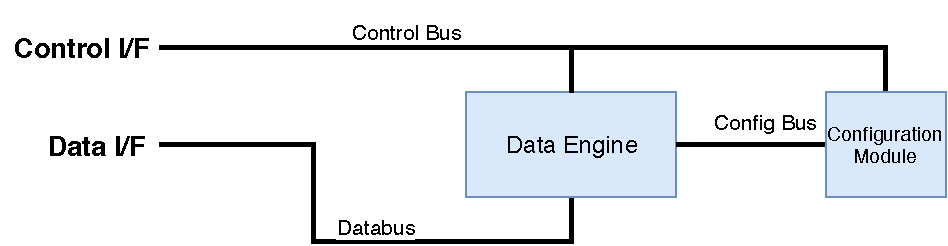
\includegraphics[width=0.80\columnwidth]{top.pdf}
\caption{Versat top-level entity.}
\label{fig_top}
\end{figure}

Versat has a DMA module so it can independently and efficiently
transfer data, programs and configurations in and out of the
device. The DMA drives a master Advanced Extensible Interface --
AXI4. It is an interface designed by ARM, which derives from the
Advanced Microcontroller Bus Architecture (AMBA).

To communicate with the host processor, Versat has a shared Control
Register File (CRF). The CRF has two host interfaces that can be
selected at compile time: a Serial Peripheral Interface (SPI) and a
parallel bus interface. The SPI slave interface is used when the host
system is an off-chip master device. The SPI interface is mainly used
for debug and testing purposes. The parallel bus interface is used
when the host is some embedded processor and may be supplied in the
AXI4 Lite format.


%%%%%%%%%%%%%%%%%%%%%%%%%%%%%%%%%%%%%%%%%%%%%%%%%%%%%%%%%%%%%%%%%%%%%%%%
\subsection{Data Engine}
\label{section:dataEngine}

The Data Engine (DE) has a fixed topology comprising 15 Functional
Units (FUs) as shown in figure~\ref{fig_de}. The DE is a 32-bit
architecture and contains the following configurable FUs: 4 dual-port
embedded memories ($8kB$ each), 6 Arithmetic and Logic Units (ALUs), 4
multipliers and 1 barrel shifter. The output register of the FUs and
the embedded memories are accessible by the Controller for reading and
writing. (The embedded memory blocks are treated like any other FU by
the Versat tools.)

\begin{figure}[!h]
\centering
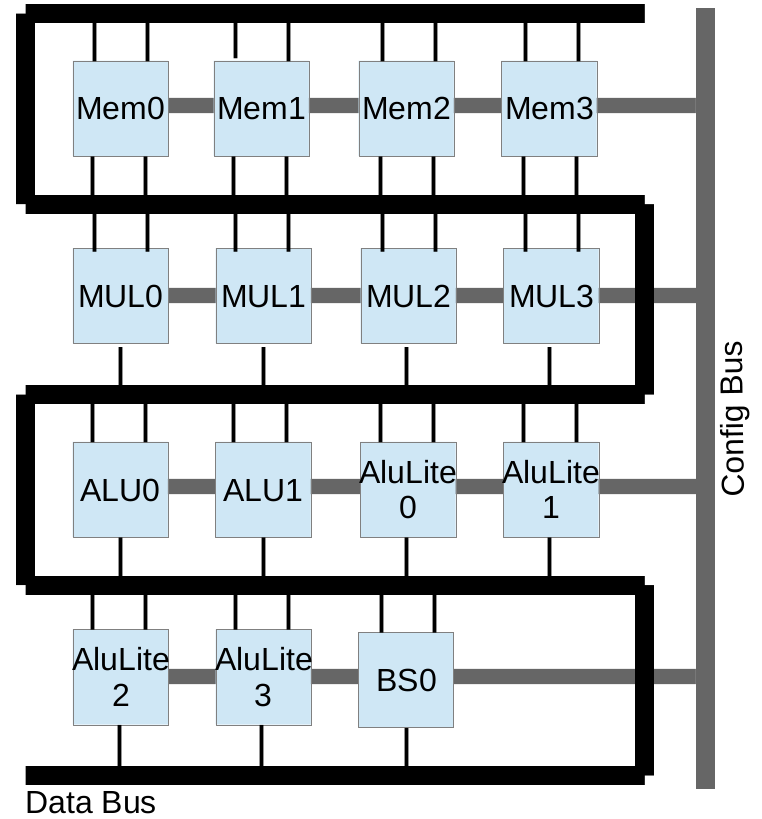
\includegraphics[width=0.85\columnwidth]{de.pdf}
\caption{Data engine.}
\label{fig_de}
\end{figure}

\subsubsection{DE Structure}
\label{subsection:DEStructure}

In the DE, the FUs are interconnected by a wide bus called the Data
Bus. The Data Bus is simply the concatenation of all FU outputs. Each
FU output contributes a 32-bit section to the Data Bus, except the
embedded memories that contribute 2 sections with their 2
ports. According to the number of FUs of each type given before, the
Data Bus has $2\times4+6+4+1=19$ sections of 32 bits. In addition to
FU outputs, the Data Bus has 2 fixed sections containing the constants
0 and 1, which have been added because they are commonly used in
datapaths. Each FU input can select any of these sections and there is
also a selection that ignores the input value so that FU can be used
as a Controller shared register. The FUs take their configurations
from the respective configuration registers in the CM, whose outputs
are concatenated in another wide bus denoted the Config Bus. There is
a fixed set of high-level operations available in each FU. For
example, an ALU can be configured to perform addition, subtraction,
several logical functions, maximum, minimum, among others.

In figure~\ref{fig_fu}, it is shown in detail how a particular FU is
connected to the control, data and configuration buses. The FU, of
type ALU, is labeled FU5 and has 2 pipeline stages. The last pipeline
stage, denoted {\tt pipeline register 1}, stores the output of the
ALU, drives one section of the Data Bus and can be read or written by
the Controller using the Control Bus (as shown in the figure). This
feature enables the FUs to be used as Controller/DE shared
registers. Each FU5 input has a programmable multiplexer to select one
of the 19 sections of the Data Bus. Although the Config Bus is shown
going to all FUs, in fact only the configuration bits of each FU are
routed to it. These bits are called the {\em configuration space} of
the FU. The configuration space is further divided in several {\em
  configuration fields}, which are 3 in this example: the selection of
input A (5 bits), the selection of input B (5 bits) and the selection
of the function (4 bits). The partial reconfiguration scheme works at
the field level, so it is only possible to reconfigure these fields
individually.

\begin{figure}[!h]
\centering
\includegraphics[width=0.85\columnwidth]{FU.pdf}
\caption{Functional unit detail.}
\label{fig_fu}
\end{figure}

Since any FU can select any FU output as one of its inputs, then the
DE has a {\em full mesh topology}. This may seem exaggerated and
unnecessary but this topology accomplishes 2 major goals: (1) {\em an
  intuitive assembly programmer's model is achieved}; (2) {\em the
  compiler design is greatly simplified}. In fact, assembly
programmers need not remember or check what is connected to what since
everything is connected to everything. Hardware datapaths can be
manually built using store instructions that write to the
configuration fields of the used FUs. A compiler can be developed with
less effort as complex place and route algorithms, commonly used in
CGRAs, become unnecessary with a fully connected topology.

Assembly programmability is a powerful feature. It may be used to
optimize critical program sections or to work around bugs. In fact,
hardware bugs, defects or failures may eventually be circumvented at
post-silicon time using assembly code to avoid using the troubled
parts of the architecture. Compiler problems can also be fixed by
replacing the failing high-level code with assembly code.

In other approaches, such as in~\cite{Mei05}, a full mesh topology
would be problematic because of the cycle by cycle reconfiguration. It
causes frequent switching of the interconnect network and consequent
power dissipation. However, in Versat, reconfiguration does not happen
every clock cycle. The interconnect consumes very little power since
Versat is reconfigured only after a complete program loop or two
levels of nested loops are executed in the DE. It may also be argued
that a full mesh topology is large and limits the frequency of
operation. However, our Integrated Circuit (IC) implementation results
indicate that only $4.04\%$ of the core area is occupied by the full
mesh interconnect, while the core can work at a maximum frequency of
$170MHz$ in a $130nm$ process. This is sufficient for many target
applications. For example, in the multimedia space, some applications
are required to work at an even lower frequency because of power and
energy constraints.

Each configuration of the DE can implement one or more hardware
datapaths. Multiple datapaths operating in parallel realize
Thread-Level Parallelism (TLP). Datapaths having identical parallel
paths implement Data-Level Parallelism (DLP). Finally, datapaths
having long FU pipelines exploit Instruction-Level Parallelism (ILP).

In figure~\ref{fig_de_dp}, three example hardware datapaths are
illustrated. Datapath (a) implements a pipelined vector
addition. Despite the fact that a single ALU is used, ILP is being
exploited as the memory reads, addition operation and memory write are
being executed in parallel for consecutive elements of the
vector. Datapath (b) implements a vectorized version of datapath (a)
to illustrate DLP combined with the ILP. The vectors to be added
spread over memories M0 and M2, so that 2 additions can be performed
in parallel. ILP and DLP can be further exploited as in datapath (c),
whose function is to compute the inner product of two vectors: four
elements are multiplied in parallel and the results enter an adder
tree with an accumulator at the root. When an ALU is used as an
accumulator the unused data input is used as a control input. As seen
in the figure, this input is kept with the value 0, which specifies
the accumulator function. Any positive value specifies this function
while a negative value specifies that the ALU simply registers the
data input.


\begin{figure}[!h]
\centering
\includegraphics[width=\columnwidth]{datapaths.pdf}
\caption{Data engine datapaths.}
\label{fig_de_dp}
\end{figure}

%%%%%%%%%%%%%%%%%%%%%%%%%%%%%%%%%%%%%%%%%%%%%%%%%%%%%%%%%%%%%%%%%%%%%%%%
\subsubsection{Address Generation Unit}
\label{subsection:addressGenerationUnit}

Versat has 4 dual-port Random Access Memories (RAMs) of size 2048
words by 32 bits, which work normally as vector registers. Each port
has an input, an output and an address input equipped with an Address
Generation Unit (AGU), as shown in figure~\ref{fig_dpram}. The AGUs
can be programmed to generate an address sequence for accessing data
from the memory port during the execution of a program loop. Our AGU
scheme is similar to the one described in~\cite{Farahini14}, in the
sense that both schemes use parallel and distributed AGUs. The AGUs
support two levels of nested loops, with the restriction that the
inner loop has a maximum of 32 iterations and the outer loop has a
maximum of 2048 iterations. To compute longer loops reconfiguration is
needed. AGUs can start execution with a programmable delay, so that
circuit paths with different accumulated latencies can be
synchronized. Each AGU can be operated independently from the other
AGUs, which allows TLP in the DE.

\begin{figure}[!h]
\centering
\includegraphics[width=0.45\columnwidth]{dpram.pdf}
\caption{Dual-port embedded memory with AGUs.}
\label{fig_dpram}
\end{figure}

Datapath (b) in figure~\ref{fig_de_dp}, previously used to explain
DLP, can also be used to explain TLP as follows. Suppose one block of
vector elements to be added is placed in memory M0, and that its
address generators M0-A, M0-B and M1-A are started (Thread 1). In
parallel, one can move the next block to memory M2 and start AGUs
M2-A, M2-B and M1-B (Thread 2). The user program can monitor the
completion of these threads and restart them with new vector
blocks. In this way, vectors that largely exceed the capacity of the
DE memories can be processed in a continuous fashion.

The AGU parameters control the generation of address sequences and
are described in~\cite{Lopes2017}. An example address sequence is
shown in figure~\ref{fig_addrgen}. Note that the AGU is enabled with a
Delay of 2 clock cycles. It is enabled periodically for $Duty=3$
cycles after every $Per=5$ cycles. The initial value of the sequence
is given by $Start=10$ (in decimal notation). Every enabled cycle it
is incremented by $Incr=2$; in the last cycle of a period it is
incremented by $Incr+Shift=-3$. This pattern repeats for $Iter$
iterations, though this parameter is not illustrated in the figure.

\begin{figure}[!h]
\centering
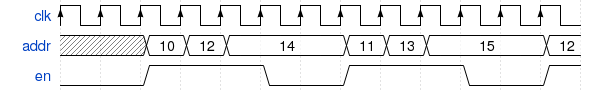
\includegraphics[width=\columnwidth]{addrgen.png}
\caption{AGU output for $Delay=2$, $Per=5$, $Duty=3$, $Start=10$, $Incr=2$, and $Shift=-5$.}
\label{fig_addrgen}
\end{figure}

The embedded memory ports have their own configuration fields: one for
selecting/disabling the input or outputting the generated sequence
(sel) and another for bypassing the AGU (Ext). If the input is
disabled then the port is enabled for reading. If it is selecting a
data source, then it is enabled for writing but also reads the word
previously stored at that address. Normally an AGU is used for
generating an address sequence for the memory port. However, the port
can also be configured to output the generated sequence to the DE,
where it can be used for general purposes. With this feature, data
patterns, synchronization and control signals can be generated for the
FUs. The configuration for bypassing the AGU ($Ext=1$) enables the
port to use as address values computed by datapath. In this case the
port address is input by the other port of the same memory. This
feature provides Versat with the capability of working with pointers.

In summary, the two memory ports can be independently configured to
read and/or write the memory, each memory port can be read/written with
an address sequence computed by the AGU or by some datapath in the
DE, and a memory configured for writing also reads the previously
stored word from the same address with one clock cycle of latency.

%%%%%%%%%%%%%%%%%%%%%%%%%%%%%%%%%%%%%%%%%%%%%%%%%%%%%%%%%%%%%%%%%%%%%%%%
\subsubsection{Arithmetic and Logic Unit}
\label{subsection:arithmeticLogicUnit}

There are two types of Arithmetic and Logic Units (ALUs), denoted Type
I and Type II: 2 Type I and 4 Type II. Both types have two inputs, A
and B, and an output Y. The ALUs have 4 configuration bits for the
operation field and thus can support 16 different
operations~\cite{Lopes2017}.

Type II ALUs use one of the configuration bits to create an internal
feedback loop from the output to input A. With the other 3 bits, Type
II ALUs can support 8 operations. If the feedback bit is set to '0',
these operations are the same as for Type I ALUs. If the feedback bit
is set to '1', the operation has input B and the current output as
operands. In this case, input A becomes available for runtime control
of the ALU, which is used for implementing conditional statements in
operations ADD, SUB, MUX, MIN and MAX. For instance, the addition
operation (ADD) can be turned into a conditional accumulate operation:
the ALU accumulates the values coming to input B, if input A is not
negative or simply registers input B otherwise. In another example,
the signed minimum operation can be used to detect and register the
minimum value among only certain elements of a sequence coming to
input B, by using input A as a data qualifier. Often, an AGU is used
to generate control sequences for the control input A of an ALU. The
type II ALU is an original way to enable conditional execution in the
DE.

%%%%%%%%%%%%%%%%%%%%%%%%%%%%%%%%%%%%%%%%%%%%%%%%%%%%%%%%%%%%%%%%%%%%%%%%
\subsubsection{Multiplier and Barrel Shifter}
\label{subsection:multiplierBarrelShifter}

The multiplier produces a 64-bit result from two 32-bit operands and
has two configuration parameters. One parameter allows selecting the
lower or higher 32 bits of the result. The other parameter forces the
multiply result to be left shifted by 1 bit. This configuration is
useful when operands are in the Q1.31 fixed-point format, which is
used in many DSP algorithms. By setting the first parameter to select
the high part of the result and the second parameter to left shift it
by 1, the multiplication of two Q1.31 operands also yields a Q1.31
result.

The barrel shifter can perform left and right shifts. Right shifts can
be configured as logical (no sign extension, feed '0' to the left) or
arithmetic (with sign extension). One configuration parameter
determines the shift direction (left or right) and another parameter
sets the right shift type (arithmetic or logic). In one input of the
barrel shifter is the value to be shifted and in the other input is
the shift size (0 to 31).

%%%%%%%%%%%%%%%%%%%%%%%%%%%%%%%%%%%%%%%%%%%%%%%%%%%%%%%%%%%%%%%%%%%%%%%%
\subsubsection{Functional Unit Latencies}
\label{subsection:functionalUnitLatencies}

Each FU has a latency due to pipelining: 2 clock cycles for the ALUs,
3 for the multipliers and 1 for the barrel shifter and embedded
memories. When configuring a datapath in the DE, it is necessary to
take into account the latency of each branch, and compensate for any
mismatches when branches with different latencies converge. To do
this, the AGUs have the {\em Delay} parameter explained
in~\cite{Lopes2017}. The branch latency is the sum of its FU
latencies.

%%%%%%%%%%%%%%%%%%%%%%%%%%%%%%%%%%%%%%%%%%%%%%%%%%%%%%%%%%%%%%%%%%%%%%%%
\subsubsection{Data Engine Control}
\label{subsection:dataEngineControl}

The DE is controlled using its Control and Status registers. The
Control register structure is the following: bit 0 (init) resets the
selected memory ports and bit 1 (run) enables the selected ports,
resets the selected FUs and starts the DE; bits~2~-~20 select the
memory ports and FUs to reset or enable. Recall there are 8 memory
ports and 11 other FUs in a total of 19 FUs to control. The Status
register structure is the following: bits~0~-~7 indicate which AGUs
are running (logic '0') or idle (logic '1').

%%%%%%%%%%%%%%%%%%%%%%%%%%%%%%%%%%%%%%%%%%%%%%%%%%%%%%%%%%%%%%%%%%%%%%%%
\subsection{Configuration Module}
\label{section:configuration}

The Configuration Module (CM) is composed of a Configuration Register
File used to prepare the next configuration, the Configuration Shadow
Register which holds the configuration being executed by the DE, and
the Configuration Memory where frequently used configurations are
stored (figure~\ref{fig_conf}). Configurations stored in the
configuration memory can later be used without modifications or they
can be partially reconfigured before used.

The configuration register file is divided in configuration spaces
which in turn are divided in configuration fields. Different
configuration spaces differ on the number of fields and configuration
fields differ on the number of bits. A full DE configuration is 672
bits. The configuration register file is addressable at the
configuration field level and there are 118 configuration fields. This
feature takes advantage of the fact that in most applications there is
a high likelihood that a certain configuration or a similar one will
be reused (time locality) to make partial reconfiguration effective.

The configuration shadow register holds an active configuration word
for the DE, which is copied from the configuration register file
whenever the Update signal is asserted by the Controller. Thus, the
contents of the configuration register file can be changed while the
configuration shadow register keeps the DE configured and running.

\begin{figure}[!h]
\centering 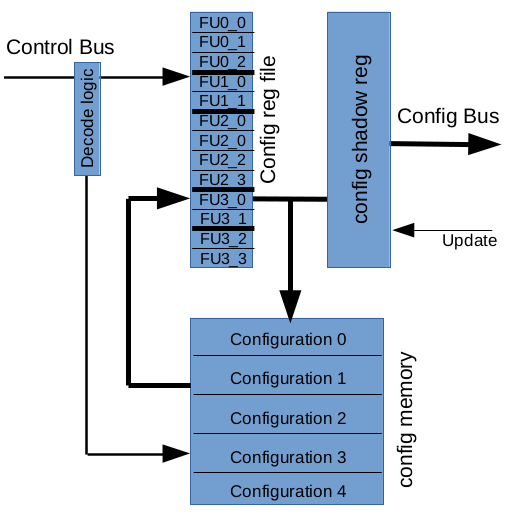
\includegraphics[width=0.85\columnwidth]{conf.pdf}
\caption{Configuration Module.}
\label{fig_conf}
\end{figure}

The configuration memory is a dual-port 64-position memory, where each
position can store a full configuration and is, hence, 672 bits
wide. Configurations can be loaded/stored from/to the configuration
register file in just 1 clock cycle using one the memory ports. The
other port is 32-bit wide and used to load and store configurations in
the external memory using the DMA. This way, the configuration memory
can be extended beyond the 64 configurations. This scheme is designed
so that one can study the difference between working with pre-built
configurations stored in external memory and generating configurations
using the Versat controller.

%%%%%%%%%%%%%%%%%%%%%%%%%%%%%%%%%%%%%%%%%%%%%%%%%%%%%%%%%%%%%%%%%%%%%%%%
\subsection{Controller}
\label{section:controller}

The Versat Controller has a minimal architecture
(figure~\ref{fig_control}) to support reconfiguration, data movement,
algorithm control and host interaction. It contains 3 main registers:
the Program Counter (PC), the Accumulator Register (RA) and the
Address Register (RB). The PC contains the address of the next
instruction as usual. Register RA is the destination of all operations
that the controller performs, and is also often one of the operands
(accumulator architecture). Register RB is addressable by the
Controller and is used to store addresses for implementing indirect
loads and stores.

\begin{figure}[!h]
\centering 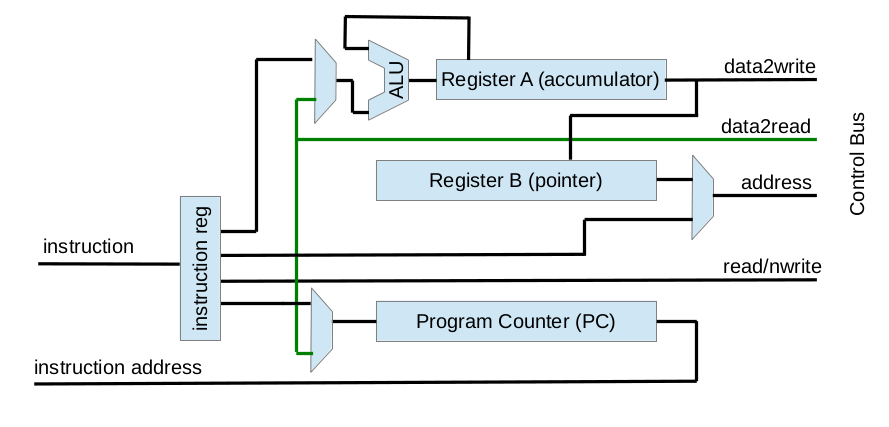
\includegraphics[width=\columnwidth]{control.pdf}
\caption{Controller.}
\label{fig_control}
\end{figure}

The controller has an instruction set of only 16 instructions (opcode
of 4 bits and {\tt Imm}ediate value of 16
bits)~\cite{Lopes2017}. These allow the controller to perform the
following actions: loads/stores to/from the accumulator,
arithmetic/logic operations and branches. There are three types of
load instructions: of immediate constants, direct (from an immediate
address) and indirect from an address stored in register RB. Store
instructions can be direct or indirect.

In order to reduce the critical path and increase the clock frequency,
a pipeline register has been added between the instruction memory and
the instruction decoder. The controller then takes 2 clock cycles to
fetch an instruction, one from the memory itself and the other from
the instruction register shown in figure~\ref{fig_control}. For
simplicity, it executes every instruction fetched and thus branch
instructions have 2 delay slots. The delay slots can be filled with
useful instructions or with no operation (NOP) instructions.  For
instance, in a {\tt for} loop, the delay slots can be used to
increment the iteration count.

The boot loader software handles host procedure calls. The host writes
the procedure parameters to the CRF and writes the program address to
R0 which triggers a jump to the program address. During the execution
of a typical program, the DMA and the DE are used multiple times. DMA
and DE threads are spawned, hiding part of the controller execution
time, as shown later. This architecture allows programs to execute
precise time delays using a {\tt for} loop with a variable number of
instructions in its body. These instructions may be useful ones
(reconfiguration instructions, for instance) or just NOP instructions.


%%%%%%%%%%%%%%%%%%%%%%%%%%%%%%%%%%%%%%%%%%%%%%%%%%%%%%%%%%%%%%%%%%%%%%%%
\subsection{DMA}
\label{section:dma}

One of the crucial factors to guarantee acceleration is the rapidity
at which data is moved in and out of Versat. Accessing data words from
the external memory using load instructions is out of the
question. Data must be moved in large blocks using a DMA engine to
amortize the latency of the external memory device. The DMA engine is
operated by the Versat controller and transfers a data burst from
external memory into one of the Versat's memories (instruction,
configuration, or data engine memory) or vice versa.

From a Versat program point of view, the DMA is memory mapped and the
following DMA registers can be accessed: the external address
register, the internal address register, the size register, the
direction register, the status register and the start register. All
registers, except the status register, are duplicated allowing the
configuration of a new transaction while a previous one is
running. The external address register holds the transfer start
address in the external memory (32 bits), and the internal address
register holds the transfer start address in Versat (14 bits written
to a 32-bit register). The size register (8 bits) specifies the number
of words to be transferred (256 words maximum, as per the AXI4
interface). The direction register indicates if the transfer is from
Versat to external memory or vice-versa. After these registers have
been configured, the program writes anything to the start register and
the transfer begins. The contents of the status register tells the
program whether the DMA is still busy, done or if an error has
occurred.

%%%%%%%%%%%%%%%%%%%%%%%%%%%%%%%%%%%%%%%%%%%%%%%%%%%%%%%%%%%%%%%%%%%%%%%%
\subsection{Program memory}
\label{section:programMemory}

The Program Memory is divided in two parts: the boot ROM (256x32,
$1kB$) and the instruction memory RAM (2048x32, $8kB$). They are
addressable as a single memory: the first 256 addresses are used to
address the boot ROM, while the others are used to address the
instruction memory.

The boot ROM holds the code that allows Versat to communicate with the
host processor. Basically, it is used for the host to call Versat
kernels and to load/store values in any addressable memory position
within Versat without using the DMA. This includes loading programs
issuing store instructions to the Program Memory. However, the Program
Memory can not be read with load instructions. Its contents can only
be executed.

%%%%%%%%%%%%%%%%%%%%%%%%%%%%%%%%%%%%%%%%%%%%%%%%%%%%%%%%%%%%%%%%%%%%%%%%
\subsection{Control Register File}
\label{section:controlRegisterFile}

The 16x32 Control Register File (CRF) is implemented with a dual-port
register file (one port for the host and another for Versat). These
registers are shared between the host processor and Versat, which are
allowed to asynchronously read or write them.


\section{Programming}

Versat can be programmed using a C/C++ subset, and the code can be
compiled using the Versat compiler~\cite{Santiago2016}. Versat can
also be programmed in assembly language, given its easy to apprehend
structure. To the best of our knowledge, Versat is the only CGRA that
can be programmed in assembly.

The user also needs a driver for the host system in order to be able
to call Versat procedures. The driver consists of only a few functions
for managing Versat. The driver and a program that uses is are
explained in detail in~\cite{Lopes2017}. The reduced number of
functions present in the driver makes Versat very easy to use by host
processors. This is mainly because Versat is independent, can
reconfigure itself, access data from the external memory and run
simple control algorithms. However, Versat needs to be programmed
separately.


\section{Results}
\label{sec:results}

In this section, experimental results for the Versat architecture are
presented and discussed. First, the implementation results for Versat
in ASIC technology are presented. Then, performance and energy
consumption results, both for simple and more complex computational
kernels, are given.

% ----------------------------------------------------------------------
\subsection{ASIC implementation results}
\label{section:ASICresults}

Versat has been designed using a UMC $130nm$ process. Here, Versat is
compared with a state-of the-art embedded processor (ARM Cortex A9)
and two other CGRA implementations (Morphosys~\cite{Lee00} and
ADRES~\cite{Mei05}). The cores are compared in terms of silicon area
({\em Area} in mm\textsuperscript{2}), embedded memory ({\em RAM} in
kB), frequency of operation ({\em Freq.} in MHz) and power consumption
({\em Power} in mW). The Versat frequency and power results have been
obtained using the Cadence IC design tools, and the node activity rate
extracted from simulating an FFT kernel. Because the different designs
use different technology nodes, in order to facilitate the
comparisons, the results are scaled to the $40nm$ technology node and
presented in Table~\ref{tabASICrs}. The scaling is performed as
explained in~\cite{borkar99}.

\begin{table}[!h]
  \begin{center}
    \begin{tabular}{lcccc}
      Core & Area & RAM &  Freq. & Power\\
      \hline
      ARM Cortex A9~\cite{wang} &  4.6 & 65.54 & 800 & 500 \\
      Morphosys~\cite{Lee00}    & 2.19 &  6.14 & 875 & 800 \\
      ADRES~\cite{Mei05}        & 0.79 & 65.54 & 675 &  40 \\
      Versat                    & 0.49 & 46.34 & 553 &  41 \\
      \hline
    \end{tabular}
  \end{center}
  \caption[Table caption shown in TOC]{ASIC implementation results scaled to $40nm$.}
  \label{tabASICrs}
\end{table}

The results show that Versat is the smallest core, and compared with
the ARM processor it is $9\times$ smaller. The ADRES architecture is
about twice the size of Versat and Morphosys is much larger, about
half the size of the ARM processor. These differences can be explained
by the different capabilities of these cores. While Versat has a
16-instruction controller and 11 FUs (excluding the memory units),
ADRES has a VLIW processor and a 4x4 FU array, and Morphosys has a
RISC processor and an 8x8 FU array.

In terms of embedded memory, Versat uses somewhat less memory than the
ARM Cortex A9 or ADRES cores, but its memory size ($46kB$) can be
considered typical for an embedded processor. Morphosys uses a lot
less memory, as it is designed to focus more on processing power and
less on storage capabilities.

The ARM core operation frequency can be considered low as this is a
power optimized version. Other versions of this core operating at
higher frequencies exist, but the area footprint is larger and the
power consumption is higher. Those versions are optimized for
performance rather than power. Among the three CGRAs, Versat is the
least optimized in terms of the working frequency. In fact, not too
much effort has been put into achieving timing closure for a higher
frequency. Notwithstanding, after analyzing the critical paths, it
became clear that there is plenty of room for optimization, so its
frequency can be considered comparable to the other CGRAs.

As far as power is concerned, Morphosys consumes more than the ARM
core. Again, this is the result of focusing in performance with a
large array of FUs. The ADRES architecture seems well optimized for
power, in spite of its cycle by cycle and progressive reconfiguration
scheme. However, the acceleration that can be achieved with ADRES is
not clearly documented in its publications~\cite{Mei05}. Versat
consumes about the same power as the ADRES core, but there is also
room for improvement, given the little effort spent so far in
low-level power optimization.

% ----------------------------------------------------------------------
\subsection{Execution results}
\label{section:executionResults}

In this subsection, Versat is compared with a state-of the-art
embedded processor in terms of performance and energy comsumption by
running a set of example kernels on Versat and on the embedded
processor. The results are divided in two parts: simple and complex
kernels. In the simple kernels part, all tests operate on vector sizes
of 1024, while in the complex kernels part, larger data sets are
used. All data is in 32-bit fixed-point format. A hardware timer has
been used to measure the time in elapsed clock cycles.

In order to assess the performance of the Versat architecture, the
Zybo Zynq-7000 ARM/FPGA SoC development board, featuring a Xilinx Zynq
7010 FPGA and a dual-core embedded ARM Cortex A9 system, has been
used. Versat is connected as a peripheral to the ARM system using its
AXI4 slave interface. The ARM system comprises a memory controller for
accessing an external DDR3 module. Versat can also access this memory
controller by connecting its AXI4 master interface to an appropriate
AXI4 slave interface on the ARM system. The Zybo development board has
been used only to measure the number of clock cycles for executing
each kernel. The speedup was estimated using the following equation:

\begin{equation}
Speedup = \frac{t_{ARM}\times f_{Versat}}{t_{Versat}\times f_{ARM}},
\label{eq:speedup}
\end{equation}
where $t_{ARM}$ and $t_{Versat}$ are the execution cycle count for the
ARM and Versat, repectively, and $f_{ARM}$ and $f_{Versat}$ are their
clock frequency in the $40nm$ process, according to
table~\ref{tabASICrs}. The energy ratio was estimated by multiplying
their execution time by their respective power consumption figure also
given in table~\ref{tabASICrs}:

\begin{equation}
Energy~Ratio = \frac{P_{ARM}}{P_{Versat}} \times Speedup.
\label{eq:energyRatio}
\end{equation}

% ----------------------------------------------------------------------
\subsubsection{Performance and energy consumption results for simple kernels}
\label{subsection:ResultsSimpleKernels}

Results for the set of simple kernels are summarized in
Table~\ref{tabExecR}. These kernels use a single Versat configuration
(no reconfiguration or reuse of data already in the accelerator), in
order to get base values for performance and energy consumption. In
the next subsubsection, it will be shown that with massive reconfigurations
and data reuse, performance and energy use improve significantly.

The results compare the performance of the Versat core with the
performance of the ARM Cortex A9 core. The kernels are the following:
{\tt vadd} is a vector addition, {\tt iir1} and {\tt iir2} are $1^{st}$
and $2^{nd}$ order IIR filters and {\tt cdp} is a dot (inner) product of
two complex vectors. All kernels operate on Q1.31 fixed-point data
with vector sizes of 1024.

For both systems, the program has been placed in on-chip memory and
the data in the external DDR3 memory device. The {\em ARM} column
denotes the execution cycle count for the ARM core. The {\em Versat}
column gives the total cycle count for the Versat core, including data
transfer, processing, control and reconfiguration. The {\em Control}
column gives the unhidden control and reconfiguration cycles, that is,
the number of these cycles that do not occur in parallel with the
execution of the DE or DMA. The number of FUs used (column {\em
  \#FUs}) and the code size in bytes (column {\em Code}) are also
given for each kernel. The speedup and energy ratio have been obtained
assuming the ARM and the Versat cores are running at the frequencies
and power figures given in Table~\ref{tabASICrs} for the $40nm$
technology node (equations~\ref{eq:speedup}
and~\ref{eq:energyRatio}). The speedup (column {\em SU}) is the
ARM/Versat ratio of execution times. (The execution time is given by
the cycle count divided by the frequency of operation.) The energy
ratio (column {\em ER}) is the energy spent by the ARM
processor divided by the energy spent by the Versat core. The consumed
energy is given by the execution time multiplied by the respective
power consumption figure.

\begin{table}[!h]
  \begin{center}
    \begin{tabular}{lccccccc}
      Kernel & ARM & Versat & Control & \#FUs & Code & SU & ER\\
      \hline
      {\tt vadd} & 14726 &  4517 & 36 &  4 & 152 & 2.25 & 27.44\\
      {\tt iir1} & 18890 &  7487 & 26 &  5 & 220 & 1.74 & 21.22\\
      {\tt iir2} & 24488 & 10567 & 26 & 11 & 332 & 1.60 & 19.51\\
      {\tt cdp}  & 25024 &  6673 & 26 & 14 & 408 & 2.59 & 31.59\\
      \hline
    \end{tabular}
  \end{center}
  \caption[Table caption shown in TOC]{Simple kernel results.}
  \label{tabExecR}
\end{table}

From these results the main conclusion is that while the achievable
speedups are modest, the energy gains are very significant for these
single configuration kernels. This makes Versat a very attractive
accelerator for high performance battery operated devices. The only
requisite is that the vectors are long enough to justify the transfer
of data in and/or out of Versat. Although not shown by the above
results, the data transfer time dominates. For example, the {\tt vadd}
kernel processing time is only 1090 cycles and the remaining 3427
cycles account for data transfer and control.

The number of FUs used is low for the {\tt vadd} and {\tt iir1}
kernels. The {\tt vadd} kernel could perform multiple additions in
parallel but it is not necessary as a single ALU is enough to hide the
data transfer time if streaming the vectors. If the data were already
in the DE then multiple ALUs in parallel would accelerate the
processing time. The {\tt iir2} and {\tt cdp} kernels use more FUs
as they require more computations per vector element.

The {\em Control} number of cycles is low for all examples, which
shows that the configuration of the DE can be accomplished almost
completely while the DMA is running. Configuration can also be done
while the DE is running, as will be shown in the next subsubsection where
runtime reconfiguration is considered. In any case, the configuration
overhead is low.

Given the simplicity of the examples, their code size, in the order of
hundreds of bytes, is small. Many of these simple kernels can be
placed in the $8kB$ program memory and invoked when necessary.

% ----------------------------------------------------------------------
\subsubsection{Performance and energy consumption results for complex kernels}
\label{subsection:ResultsComplexKernels}

In this subsubsection, three more complex kernels, that demand self
and partial reconfiguration, are presented. The number of
reconfigurations is high and the kernels operate for a long time on
the data fetched from the external memory and/or produced by
themselves. In these examples the data transfer time is less
significant. The chosen examples are the following
(see~\cite{Lopes2017}):
\begin{itemize}
\item 1D-Convolution (conv-1D): very popular in applications such as
  Convolutional Neural Networks;
\item Fast Fourier Transform (FFT): very common in digital signal processing;
\item K-Means Clustering algorithm (K-Means): widely used in Big Data
  applications.
\end{itemize}

These examples are {\em parameterizable} and the parameters are passed
by the host processor using the CRF. The algorithm that runs on Versat
processes the parameters and generates configurations
accordingly. This would be hard to achieve with statically compiled
configurations and demonstrates the strength of self-generated
configurations. Partial reconfigurations are equally important
since they reduce considerably the reconfiguration time.

Results for 3 particular instances of the conv-1D, FFT and K-Means
algorithms are detailed in Table~\ref{tabExecR2}. The conv-1D result
was obtained by running the kernel on a dataset of $10^6$ points
applying 1-D convolution on a 256-point sliding window. The FFT result
pertains a 16384-point window size with a $50\%$ overlap over a
dataset of $10^6$ complex points. The K-Means result has been obtained
for one iteration over a dataset of $1.36 \times 10^6$ points of 30
dimensions and 34 centroids.

\begin{table}[!h]
  \begin{center}
    \begin{tabular}{lcccccc}
      Kernel & ARM & Versat & \#FUs & Code & SU & ER\\
      \hline
      {\tt conv-1D} & 2.26G & 104.51M & 13   &  668 & 14.95 & 182.32\\
      {\tt FFT}     & 1.28G &  34.50M & 12   & 3492 & 25.65 & 312.80\\
      {\tt K-Means} & 9.02G &   1.64G & 12.5 & 2764 &  3.8  &  46.28\\
      \hline
    \end{tabular}
  \end{center}
  \caption[Table caption shown in TOC]{Complex kernel results.}
  \label{tabExecR2}
\end{table}

These results show that the speedup and energy efficiency improve with
the complexity of the kernels when compared to the simpler kernels in
the previous subsubsection. This has to do with the number of operations
done in parallel in the DE, but also with the number of DE
configurations that can be executed without fetching or saving new
data in the external memory. The K-Means algorithm fetches a new
datapoint chunk and applies 2 DE configurations: one for performing
datapoint classification and the other to update the centroid
positions. As for the FFT and conv-1D, after fetching a datapoint
chunk, several configurations are applied corresponding to the several
FFT stages, in case of the FFT and a window computation, in case of
conv-1D. The datapaths for these kernels also expose a higher ILP and
DLP in its computations. Hence, the speedup and energy efficiency of
the FFT and conv-1D are much higher when compared to the K-Means
algorithm. All these algorithms illustrate the power of using the
Versat CGRA compared to the ARM processor.

%\subsubsubsection{Conv-1D results}

In the conv-1D kernel, the only parameterizable parameter is the
window size. Versat/ARM speedup results are shown in
figure~\ref{fig:convsu}.  The window size is varied from 32 to 1024 and
is increased by powers of 2. All datapoints, from the first data
chunk, are multiplied by the sliding window coefficients and
accumulated. Then Versat reconfigures itself to advance to the next
window and the process repeats until the window is slid over all
datapoints.

\begin{figure}[!h]
  \centering \includegraphics[width=0.8\columnwidth]{speedupConv.eps}
  \caption{Conv-1D: speedup vs. window size.}
  \label{fig:convsu}
\end{figure}

As the sliding window size increases, the ARM core can better hide the
time needed to store the computed values while the Versat core keeps
its execution time linear on the window size. This causes a slight
speedup drop, from $16.3$ to $15.2$, as shown in the figure. Due to
the small size of the data chunks, the size of the internal memories
is adequate for both cores.

%\subsubsubsection{FFT results}

The FFT kernel can be parameterized with the following parameters: the
number of datapoints, window size (must be a power of 2) and window
overlap size. The algorithm computes the FFT successively, for the
points in the sliding window, advancing the window for a number of
points given by the window size minus the overlap size. In
figure~\ref{fig:fftsu}, the Versat/ARM speedup is shown as a function of
the window size for 1 million datapoints and a half window ($50\%$)
overlap.

\begin{figure}[!h]
  \centering \includegraphics[width=0.8\columnwidth]{speedup3.eps}
  \caption{FFT: speedup vs. window size.}
  \label{fig:fftsu}
\end{figure}

Initially, as the sliding window size reaches the capacity of the
Versat memories, the speedup drops, while the ARM core uses its data
cache and pre-fetch mechanism to sustain its performance. However, as
the window size further increases, the ARM core reaches its own
internal memory limitations for streaming data, and the speedup
increases steadily again after that.

%\subsubsubsection{K-means clustering results}

The parameters that can be passed to the K-Means Clustering kernel are
the following: the number of datapoints, number of dimensions and
number of centroids. In figure~\ref{fig:timeVSdpts}, it is shown how
the time for one iteration varies with the number of datapoints for a
fixed number of dimensions and centroids. The results are given for
both cores using logarithmic scales.

\begin{figure}[!h]
  \centering \includegraphics[width=0.8\columnwidth]{points.eps}
  \caption{K-Means: iteration time vs. number of datapoints, for 30 dimensions and 34 centroids.}
  \label{fig:timeVSdpts}
\end{figure}

These results show that for both systems the execution time scales
linearly with the number of datapoints. The Versat/ARM average speedup
is $3.8$, taking into account the number of clock cycles and the
working frequencies of the cores (Table~\ref{tabASICrs}). Despite the
modest speedup achieved in the K-Means Clustering algorithm, a
considerable amount of energy can be saved.

Each point requires the DE to be reconfigured twice to apply the
Assignment and Update steps. Since this algorithm is applied to
millions of points then Versat is reconfigured millions of times at
runtime. There is no reconfiguration overhead, as all reconfigurations
are done while the DE or DMA is running.

\subsubsection{Generated versus stored configurations}

To show that using self-generated configurations has advantage
compared to storing all configurations in the external memory,
consider the K-Means Clustering kernel for instance.

This algorithm is especially useful when applied to large data
sets. In the implementation above it has been chosen to apply it to
millions of datapoints. Since for this algorithm Versat
self-reconfigures for each point, then millions of configurations are
needed. Since one configuration uses 672 bits then 672Mbits are needed
only for configurations, much more than needed to store the program
itself which generates the configurations.

For algorithms that require a number of configurations tied to the
dataset size, pre-compiling and storing all configurations becomes
simply not practical. Even for the FFT kernel that only requires 43
configurations, it can be proved that the self-generated version is
marginally more efficient and has smaller memory footprint than the
stored configurations version. Therefore, self-generated
configurations is a good technique for CGRAs.


\section{Conclusion}

In this paper we have described a new Coarse Grained Reconfigurable
Array (CGRA) architecture, named Versat, and we have compared it with
some other CGRA architectures. The main difference is that Versat uses
self-generated and partial reconfiguration. These configurations are
generated by an internal controller. The controller also takes care of
data transfers to/from the external memory and simple algorithmic
control. This allows Versat to independently run complex kernels such
as the FFT and K-Means Clustering kernels.

Versat is a minimal fixed-point CGRA with 4 dual-port embedded
memories, 11 FUs, and a basic 16-instruction controller. Compared with
other CGRAs with larger arrays, Versat requires a more sophisticated
reconfiguration mechanism: the Versat controller can generate partial
configurations and writes them field by field to a fully addressable
configuration register file. The controller is also in charge of data
transfers and basic algorithmic flows. This new architecture has
several novel features: (1) one address generation unit per memory
port, tightly coupled to it; (2) pointer support as values computed in
the data engine can be used as memory addresses; (3) the address
sequences produced by the address generators can be output and used in
the data engine for any other purposes (data generators); (4) the ALUs
support conditional and cumulative functions such as the accumulate
and minimum functions, computed only if a condition is true. Feature
(3) is especially useful for generating synchronization signals for
the functional units in the data engine and feature (4) enables the
execution of loops that contain if statements in their bodies.

Versat can be programmed in two different ways: in assembly language
and using a C/C++ subset. To the best of our knowledge, Versat is the
only CGRA architecture that can be programmed in assembly
language. Assembling programmability provides ultimate control over
all architecture details and is invaluable in software optimization,
debug and system repair. Versat is designed to be a programmable
alternative to dedicated hardware accelerators, eliminating the risk
of design errors. A software driver for host processors to use Versat
has been developed.


% ----------------------------------------------------------------------
%\subsection{Achievements}
%\label{section:achievements}

Versat is $9.4\times$ smaller than an ARM Cortex A9 processor and can
achieve a $553MHz$ clock frequency, while the ARM core can run at
$800MHz$ in the same $40nm$ technology node. Performance results on
running an FFT kernel show that the Versat core can be $18\times$
faster and $220\times$ more energy efficient than the embedded
processor. Running a K-Means Clustering kernel, it is $3.8\times$
faster and consumes $46.3\times$ less energy. It should be clear from
these numbers that GPUs and FPGAs cannot compete in this arena, and
that the presented solution is useful in applications where cost and
energy consumption are crucial.

% use section* for acknowledgement

% needed in second column of first page if using \IEEEpubid
%\IEEEpubidadjcol


% An example of a floating figure using the graphicx package.
% Note that \label must occur AFTER (or within) \caption.
% For figures, \caption should occur after the \includegraphics.
% Note that IEEEtran v1.7 and later has special internal code that
% is designed to preserve the operation of \label within \caption
% even when the captionsoff option is in effect. However, because
% of issues like this, it may be the safest practice to put all your
% \label just after \caption rather than within \caption{}.
%
% Reminder: the "draftcls" or "draftclsnofoot", not "draft", class
% option should be used if it is desired that the figures are to be
% displayed while in draft mode.
%
%\begin{figure}[!t]
%\centering
%\includegraphics[width=2.5in]{myfigure}
% where an .eps filename suffix will be assumed under latex, 
% and a .pdf suffix will be assumed for pdflatex; or what has been declared
% via \DeclareGraphicsExtensions.
%\caption{Simulation results for the network.}
%\label{fig_sim}
%\end{figure}

% Note that the IEEE typically puts floats only at the top, even when this
% results in a large percentage of a column being occupied by floats.


% An example of a double column floating figure using two subfigures.
% (The subfig.sty package must be loaded for this to work.)
% The subfigure \label commands are set within each subfloat command,
% and the \label for the overall figure must come after \caption.
% \hfil is used as a separator to get equal spacing.
% Watch out that the combined width of all the subfigures on a 
% line do not exceed the text width or a line break will occur.
%
%\begin{figure*}[!t]
%\centering
%\subfloat[Case I]{\includegraphics[width=2.5in]{box}%
%\label{fig_first_case}}
%\hfil
%\subfloat[Case II]{\includegraphics[width=2.5in]{box}%
%\label{fig_second_case}}
%\caption{Simulation results for the network.}
%\label{fig_sim}
%\end{figure*}
%
% Note that often IEEE papers with subfigures do not employ subfigure
% captions (using the optional argument to \subfloat[]), but instead will
% reference/describe all of them (a), (b), etc., within the main caption.
% Be aware that for subfig.sty to generate the (a), (b), etc., subfigure
% labels, the optional argument to \subfloat must be present. If a
% subcaption is not desired, just leave its contents blank,
% e.g., \subfloat[].


% An example of a floating table. Note that, for IEEE style tables, the
% \caption command should come BEFORE the table and, given that table
% captions serve much like titles, are usually capitalized except for words
% such as a, an, and, as, at, but, by, for, in, nor, of, on, or, the, to
% and up, which are usually not capitalized unless they are the first or
% last word of the caption. Table text will default to \footnotesize as
% the IEEE normally uses this smaller font for tables.
% The \label must come after \caption as always.
%
%\begin{table}[!t]
%% increase table row spacing, adjust to taste
%\renewcommand{\arraystretch}{1.3}
% if using array.sty, it might be a good idea to tweak the value of
% \extrarowheight as needed to properly center the text within the cells
%\caption{An Example of a Table}
%\label{table_example}
%\centering
%% Some packages, such as MDW tools, offer better commands for making tables
%% than the plain LaTeX2e tabular which is used here.
%\begin{tabular}{|c||c|}
%\hline
%One & Two\\
%\hline
%Three & Four\\
%\hline
%\end{tabular}
%\end{table}


% Note that the IEEE does not put floats in the very first column
% - or typically anywhere on the first page for that matter. Also,
% in-text middle ("here") positioning is typically not used, but it
% is allowed and encouraged for Computer Society conferences (but
% not Computer Society journals). Most IEEE journals/conferences use
% top floats exclusively. 
% Note that, LaTeX2e, unlike IEEE journals/conferences, places
% footnotes above bottom floats. This can be corrected via the
% \fnbelowfloat command of the stfloats package.


% if have a single appendix:
%\appendix[Proof of the Zonklar Equations]
% or
%\appendix  % for no appendix heading
% do not use \section anymore after \appendix, only \section*
% is possibly needed

% use appendices with more than one appendix
% then use \section to start each appendix
% you must declare a \section before using any
% \subsection or using \label (\appendices by itself
% starts a section numbered zero.)
%


%\appendices
%\section{Proof of the First Zonklar Equation}
%Appendix one text goes here.

% you can choose not to have a title for an appendix
% if you want by leaving the argument blank
%\section{}
%Appendix two text goes here.


% use section* for acknowledgment
\section*{Acknowledgment}
%\begin{tiny}
This work was supported by national funds
through Funda\c c\~ao para a Ci\^encia e a Tecnologia (FCT) with
reference UID/CEC/50021/2013.
%\end{tiny}


% Can use something like this to put references on a page
% by themselves when using endfloat and the captionsoff option.
\ifCLASSOPTIONcaptionsoff
  \newpage
\fi



% trigger a \newpage just before the given reference
% number - used to balance the columns on the last page
% adjust value as needed - may need to be readjusted if
% the document is modified later
%\IEEEtriggeratref{8}
% The "triggered" command can be changed if desired:
%\IEEEtriggercmd{\enlargethispage{-5in}}

% references section

% can use a bibliography generated by BibTeX as a .bbl file
% BibTeX documentation can be easily obtained at:
% http://mirror.ctan.org/biblio/bibtex/contrib/doc/
% The IEEEtran BibTeX style support page is at:
% http://www.michaelshell.org/tex/ieeetran/bibtex/
%\bibliographystyle{IEEEtran}
\bibliographystyle{unsrt}
% argument is your BibTeX string definitions and bibliography database(s)
\bibliography{Thesis_bib_DB}
%
% <OR> manually copy in the resultant .bbl file
% set second argument of \begin to the number of references
% (used to reserve space for the reference number labels box)
%\begin{thebibliography}{1}

%\bibitem{IEEEhowto:kopka}
%H.~Kopka and P.~W. Daly, \emph{A Guide to \LaTeX}, 3rd~ed.\hskip 1em plus
%  0.5em minus 0.4em\relax Harlow, England: Addison-Wesley, 1999.
%\end{thebibliography}

% biography section
% 
% If you have an EPS/PDF photo (graphicx package needed) extra braces are
% needed around the contents of the optional argument to biography to prevent
% the LaTeX parser from getting confused when it sees the complicated
% \includegraphics command within an optional argument. (You could create
% your own custom macro containing the \includegraphics command to make things
% simpler here.)
%\begin{IEEEbiography}[{\includegraphics[width=1in,height=1.25in,clip,keepaspectratio]{mshell}}]{Michael Shell}
% or if you just want to reserve a space for a photo:



% insert where needed to balance the two columns on the last page with
% biographies
%\newpage

% You can push biographies down or up by placing
% a \vfill before or after them. The appropriate
% use of \vfill depends on what kind of text is
% on the last page and whether or not the columns
% are being equalized.

%\vfill

% Can be used to pull up biographies so that the bottom of the last one
% is flush with the other column.
%\enlargethispage{-5in}



% that's all folks
\end{document}


